%
% latex-sample.tex
%
% This LaTeX source file provides a template for a typical research paper.
%

%
% Use the standard article template.
%
\documentclass{article}

% The geometry package allows for easy page formatting.
\usepackage{geometry}
\geometry{letterpaper}

% Load up special logo commands.
\usepackage{doc}

% Package for formatting URLs.
\usepackage{url}

% Packages and definitions for graphics files.
\usepackage{graphicx}
\usepackage{epstopdf}
\DeclareGraphicsRule{.tif}{png}{.png}{`convert #1 `dirname #1`/`basename #1 .tif`.png}

%
% Set the title, author, and date.
%
\title{Dream Interface for Headmaster}
\author{Chase Blokker}
\date{11/29/12}

%
% The document proper.
%
\begin{document}

% Add the title section.
\maketitle


\section{Introduction}
\label{Introduction}

The concept for my dream interface utilizes the accelerometer found in most smart phones.  The user controls a steel ball, and tilts the phone to move the ball in the desired direction.  Menus are represented as holes.  When the ball falls into one of these holes, the menu is selected, and the page is refreshed to the related selected menu.\\

When the user starts the mobile app, the ball is positioned in the center of the screen.   The user has the option of tilting the phone in four directions to move the ball towards submenu items within students, grants, events, or reports.  When the ball goes through one of these menu “channels”, the user has selected the first level of the menu.  The ball then enters a new chamber that has the submenu items.  For example, if the user rolls the ball towards the direction of Students, the user can now select a student based off of grade by following either the freshmen, sophomore, junior, or senior channel.  Within these channels are individual students.  The user selects a student by getting the ball into the student’s hole.  The page is then refreshed to a more traditional headmaster interface, displaying all the information.\\

The design will be skeuomorphic in the sense that it will imitate a traditional ball tilt maze.  This maze was traditionally called labyrinth, and can be seen pictured below.  The object of the game is to get a steel ball from one side of the maze to the other side of the maze by avoiding all the holes.  The user moves the ball by adjusting the angle of the board.  Two nobs found on the side can move the x-axis and y-axis of the board.  Adjusting these nobs thereby move the ball.  In the phone interface, instead of using two nobs, the user can adjust the x-axis and y-axis of the phone directly to update the position of the ball.\\

This interface is prone to user error because it may be easy to accidentally get the ball in the wrong hole.

\begin{figure}[ht!]
\centering
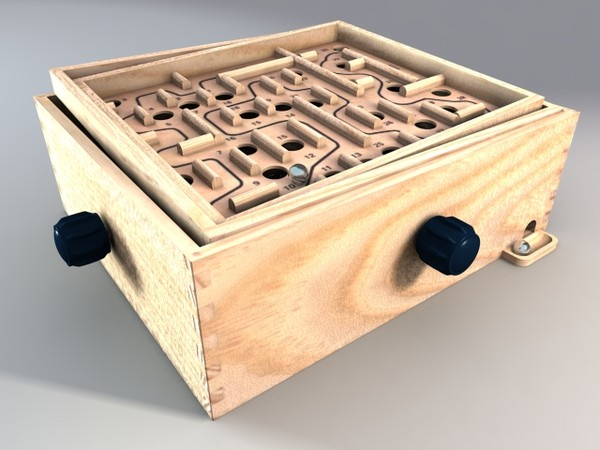
\includegraphics[width=90mm]{labyrinth.jpeg}
\caption{The game Labyrinth}
\label{overflow}
\end{figure}

\pagebreak
\


\begin{figure}[ht!]
\centering
\includegraphics[width=140mm]{example.png}
\caption{The example interface}
\label{overflow}
\end{figure}




\end{document}